In this section we investigate the performance of the MEM by applying it to synthetic Greens function in order to recover the spectrum $A(\omega)$. We generate the Greens function data by first calculating the spectrum $A(\omega)$ and then using Equ. to calculate the Greens function given our spectrum and the kernel $K(\tau,\omega)$. After that we corrupt the Greens function by Gaussian noise as the ``real'' Greens function obtained by Quantum Monte Carlo methods always suffer from noise. In this evaluation we solely use the spectrum of the BCS superconductor for our investigation which can be calculated by 
\begin{equation}
	A(\omega) = 
		\begin{cases}
			\frac{1}{W} \frac{|\omega|}{\sqrt{\omega^2 - \Delta^2}}&, \text{ if } \Delta < |\omega| < \frac{W}{2} \\
			0 &, \text{else}
		\end{cases}
	\label{results:equ.1}
\end{equation}
where $W$ denotes the bandwidth and $2\Delta$ the gap magnitude.
In Fig. we show an example of the spectrum and the resulting Greens function for $W = 0.9$ and $\Delta = 10$.
\begin{figure}[htbp]
	\centering
	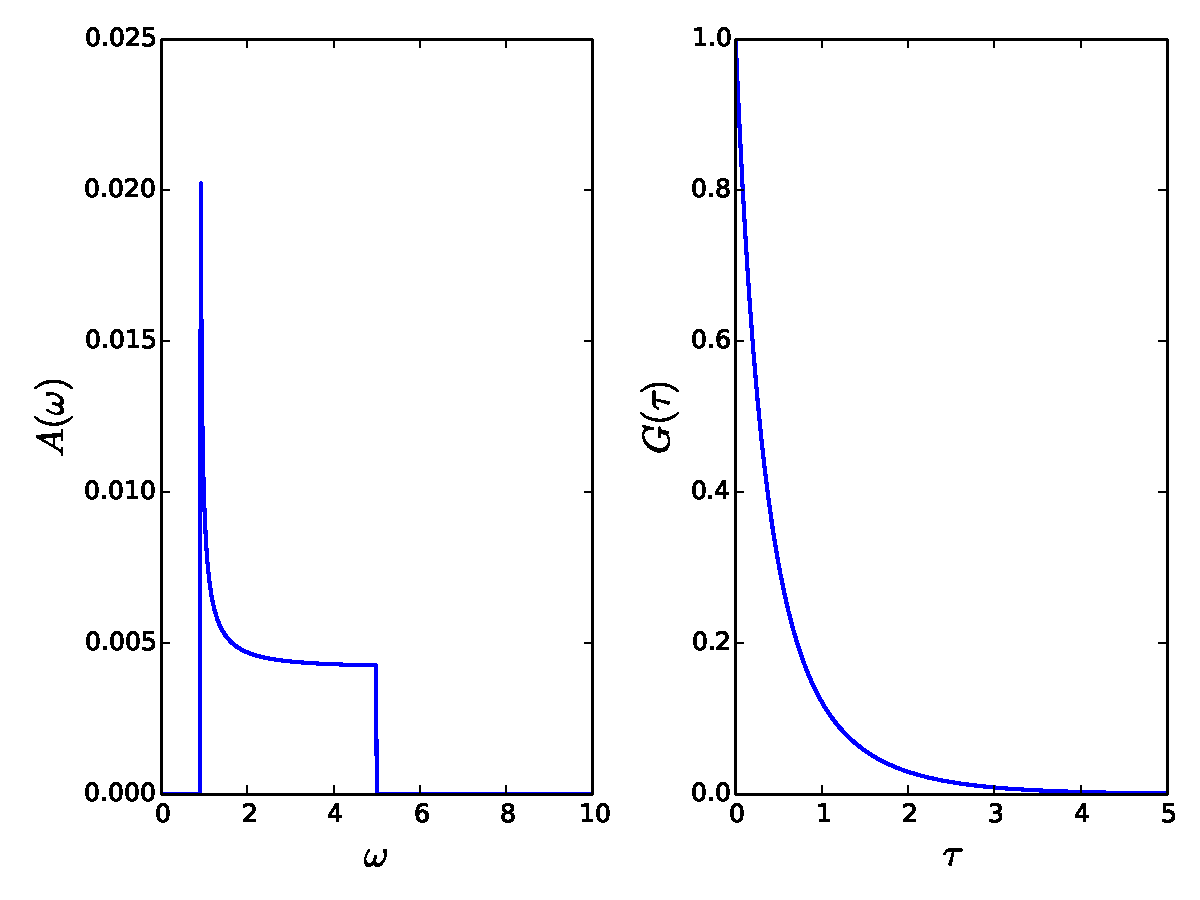
\includegraphics[width=0.95\textwidth]{./images/BCS_A_G_example.pdf}
	\caption{Example BCS spectrum $A(\omega)$ (left) and resulting Greens function $G(\tau)$ (right). The spectrum is calculated according to Equ. \ref{results:equ.1} with $\Delta = 0.9$ and $W = 10$.}
	\label{results:fig.1}
\end{figure}
\FloatBarrier
During our investigation of MEM we encountered a high numerical instability of the method. Especially for low values of $\Sigma$ the algorithm resulted in either very inaccurate results or ``crashed'' due to numerical overflow in $\vec A$. This behavior is highly counter intuitive and one should put a great thought on the data before using this formalism. As mentioned we firstly encountered a lot of numerical overflows in $\vec A$ when we used the criterion $\vec{\delta u}^T T \vec{\delta u} \leq \sum m_i$proposed by Bryan. We managed to get rid of the overflows by changing the norm used to truncate the maximum step length by using the criterion $\parallel \vec A \parallel^2 \leq \sum_i m_i$. However, this only partially solved the problem, as now the algorithm does not converge to a acceptable solution in a great number of times. At the times when Bryan proposed this algorithm and Jarrell adapted it for analytic continuation of Quantum Monte Carlo data, the accessible accuracies for the data where much lower than they are nowadays. We simply expect this to be the reason that neither Bryan of Jarrell address this issue. Therefor, we restrict ourselves to a minimum error of $10^{-4}$ for the whole investigation. \newline
The results obtained by MEM highly depend on the regularization parameter $\alpha$. We demonstrate the influence of $\alpha$ by estimating the spectrum shown in Fig. \ref{results:fig.1} for three different values for $\alpha = 0.5,2.5,10$. The results are shown in Fig. \ref{results:fig.2}
\begin{figure}[htbp]
	\centering
	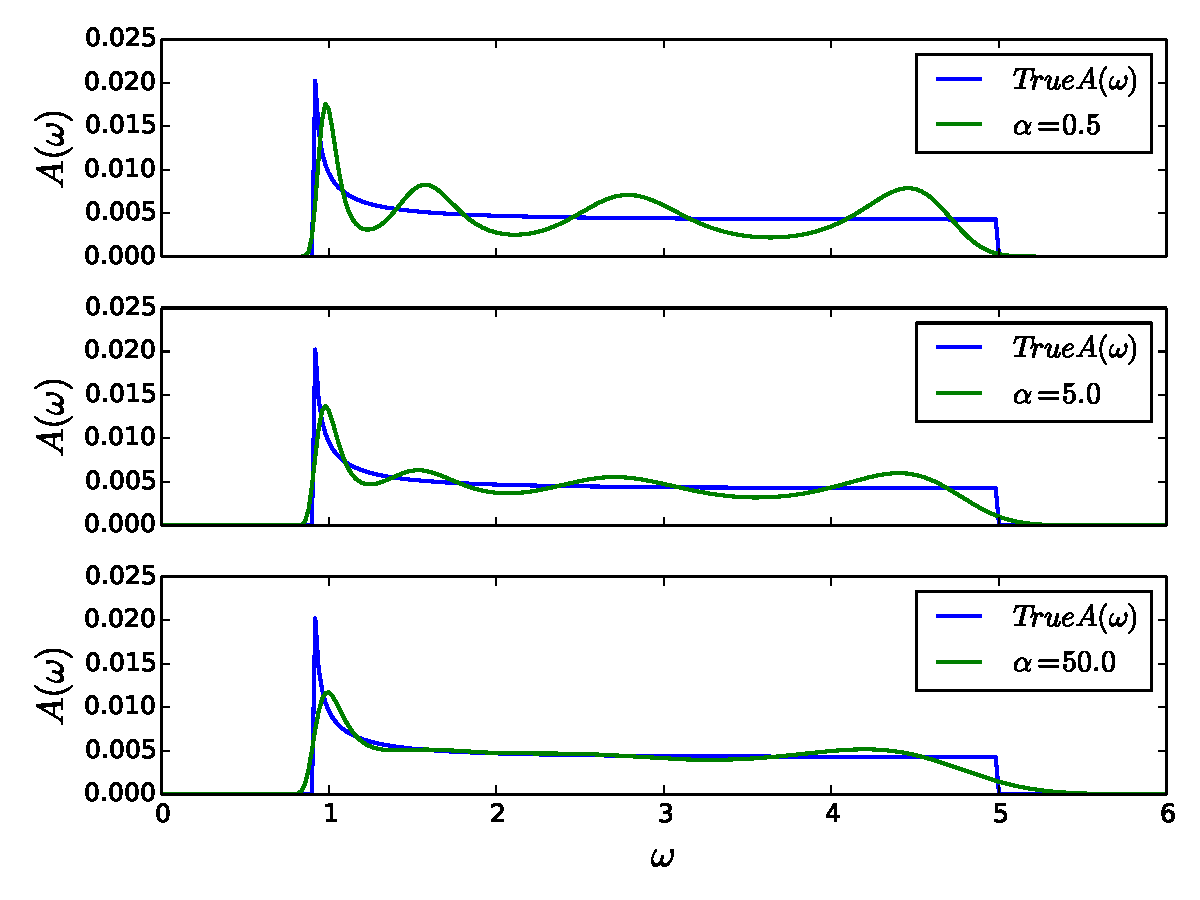
\includegraphics[width=0.95\textwidth]{./images/BCS_varying_alpha.pdf}
	\caption{Influence of the regularization parameter $\alpha$ on the performance of the Maximum Entropy method. The spectrum is calculated according to Equ. \ref{results:equ.1} with $\Delta = 0.9$ and $W = 10$.}
	\label{results:fig.2}
\end{figure}
\FloatBarrier
Another important parameter is the choice of the minimum singular value $\theta$ which determines the dimension of the singular space. We investigate the impact of $\theta$ on the performance of the Maximum Entropy method in Fig. \ref{results:fig.3}
\begin{figure}[htbp]
	\centering
	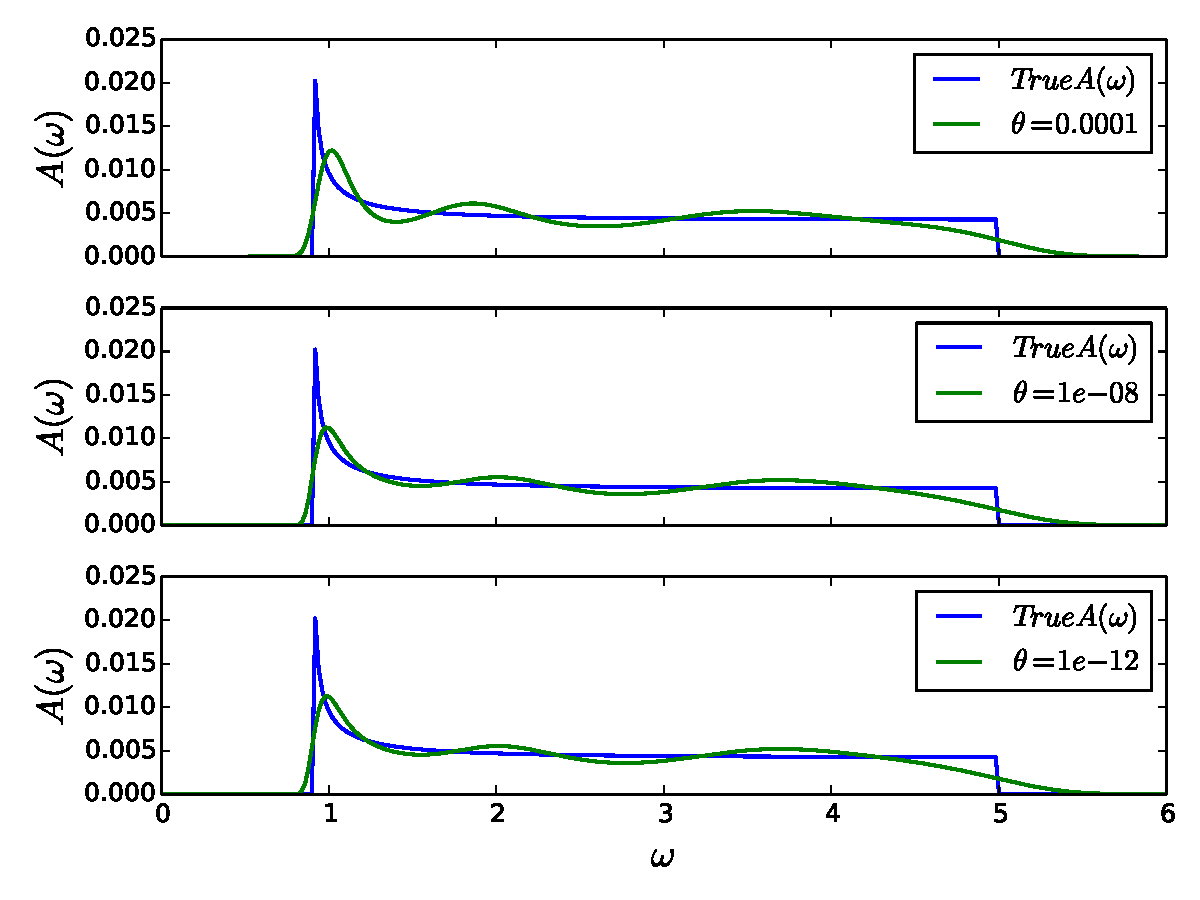
\includegraphics[width=0.95\textwidth]{./images/BCS_varying_cutoffs.pdf}
	\caption{Influence of the minimum singular value $\theta$ on the performance of the Maximum Entropy method. The spectrum is calculated according to Equ. \ref{results:equ.1} with $\Delta = 0.9$ and $W = 10$.}
	\label{results:fig.3}
\end{figure}
\FloatBarrier
Finally we show the difference between classic MEM and the Bryan method in choosing $\alpha$. As discussed in Sec. !!Reference!! the classic MEM uses the maximum value of the probability of $\alpha$ given $A$ and $G$ while Bryan calculates the final $\hat{A}$ by  $\hat{A} = \int A(\alpha) P_{\alpha} d\alpha$. In Fig. we show the probability $p_{\alpha}$ and the resulting spectra calculated by classic and Bryan's method
\begin{figure}[htbp]
	\centering
	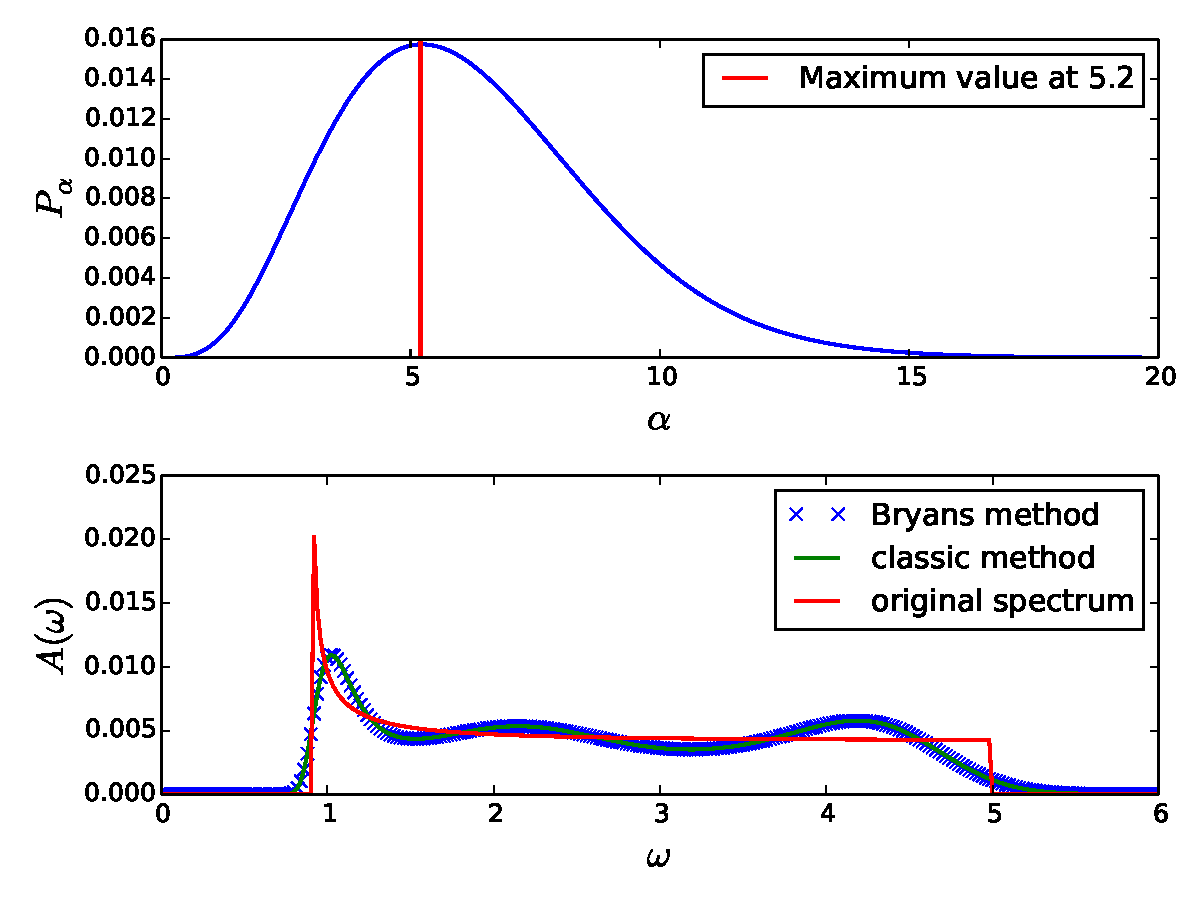
\includegraphics[width=0.95\textwidth]{./images/BCS_Bryan_classic_p_alpha.pdf}
	\caption{caption}
	\label{results:fig.4}
\end{figure}
\FloatBarrier